\documentclass[a4paper,10pt]{book}
\usepackage[utf8]{inputenc}
\usepackage{tikz}
\usepackage{hyperref}

\newcommand{\icon}[1]{\tikz[baseline=-3pt] \node[inner sep=0pt,outer sep=0pt]{\includegraphics[height=1.1em]{images/#1}};}

%opening
\title{ADAMS - Scientific Workflow Management}
\author{Peter Reutemann}

\begin{document}

\chapter{Twitter Research}
ADAMS offers a large amount of actors for a wide range of data processing and mining tasks. However, we limit ourselves here to the analysis of data obtained from Twitter. The following sections cover how to set up ADAMS in order to access Twitter, how to collect tweets for further analysis, replay collected tweets, visualize them and how to perform various analyses.

\section{Twitter setup}
ADAMS uses the twitter4j\footnote{\url{http://twitter4j.org/}{}} library for accessing twitter. In order to access some of the functionality of the Twitter API, you need to have a developer account and register an application with API key/secret and Access token/secret. You can register an application on the Twitter Developer website\footnote{\url{https://dev.twitter.com/}{}}. Figure \ref{twitter_dev} shows an example website for an ADAMS application, complete with API key/secret and Access token/secret. Once you have obtained these keys/tokens/secrets you can enter these in the ADAMS preferences for Twitter, as shown in Figure \ref{twitter_preferences}.

\begin{figure}[htb]
  \centering
  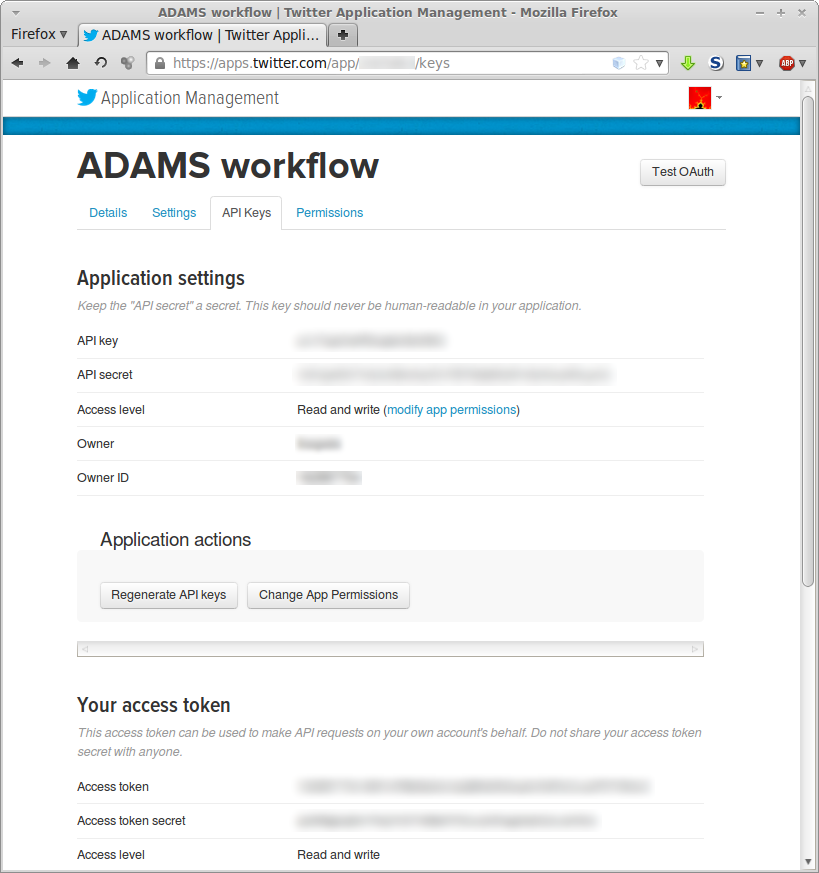
\includegraphics[width=10.0cm]{images/twitter_dev.png}
  \caption{Application management through the ``Twitter Developers'' website, displaying keys, tokens and secrets for an application.}
  \label{twitter_dev}
\end{figure}

\begin{figure}[htb]
  \centering
  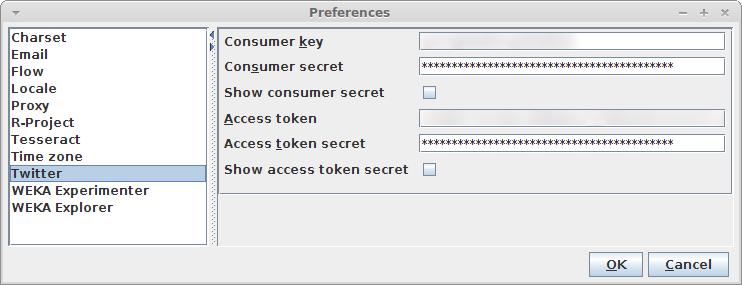
\includegraphics[width=10.0cm]{images/twitter_preferences.png}
  \caption{Preferences page for Twitter in ADAMS.}
  \label{twitter_preferences}
\end{figure}

\section{Collecting tweets}
TODO\footnote{According to Twitter's API Rules, you can collect tweets, but you are not allowed to redistribute them. See \url{https://twitter.com/apirules}{} for more details.}

\begin{figure}[htb]
  \centering
  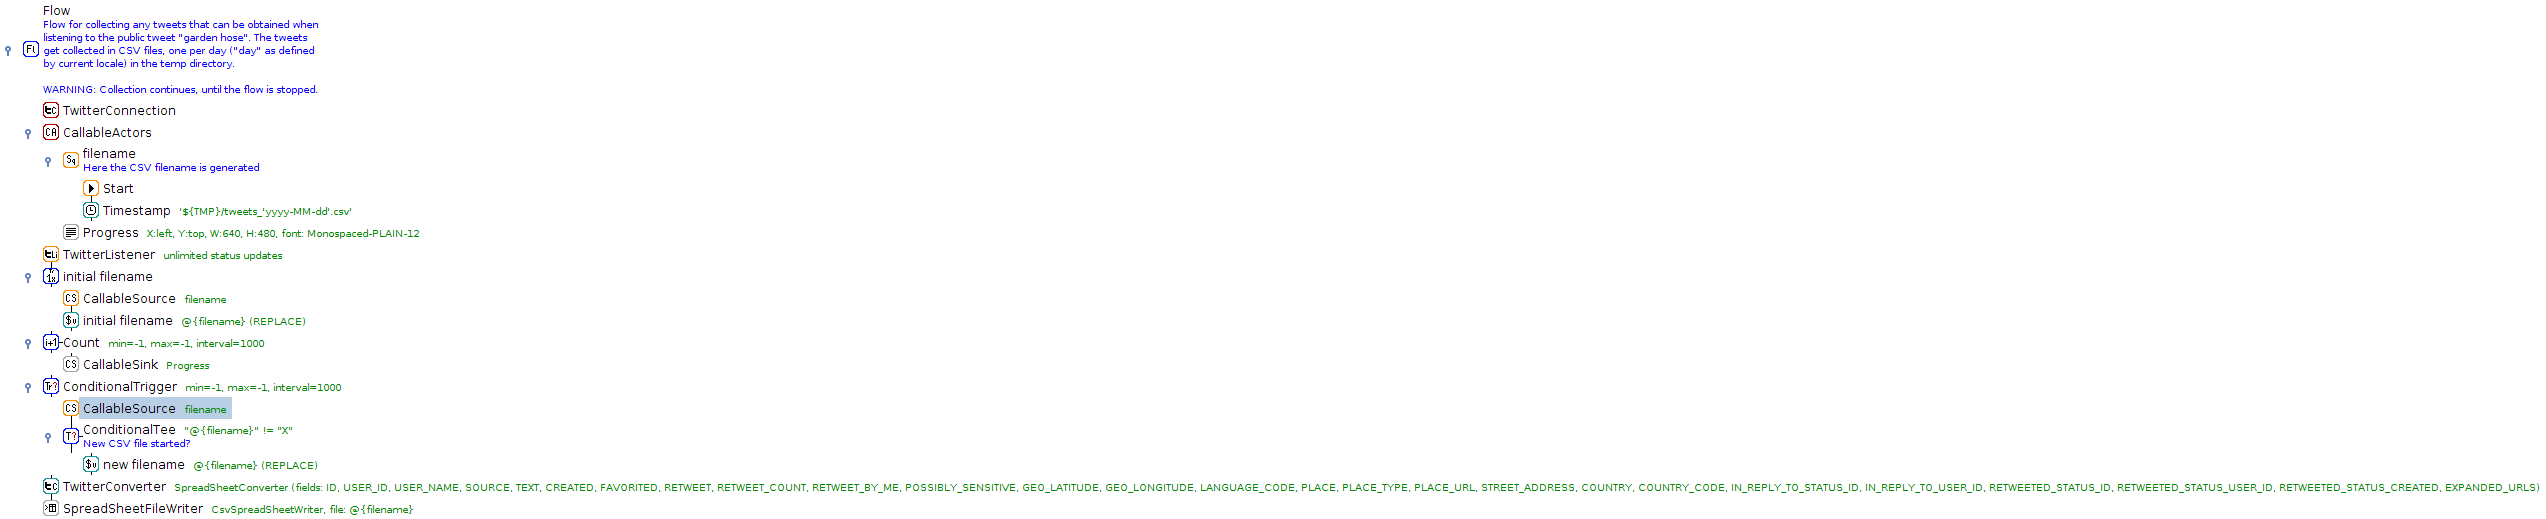
\includegraphics[width=8.0cm]{images/collect_tweets-flow.png}
  \caption{Flow for collecting tweets in CSV archive files.}
  \label{collect_tweets-flow}
\end{figure}

\section{Replaying and filtering tweets}
TODO

\begin{figure}[htb]
  \centering
  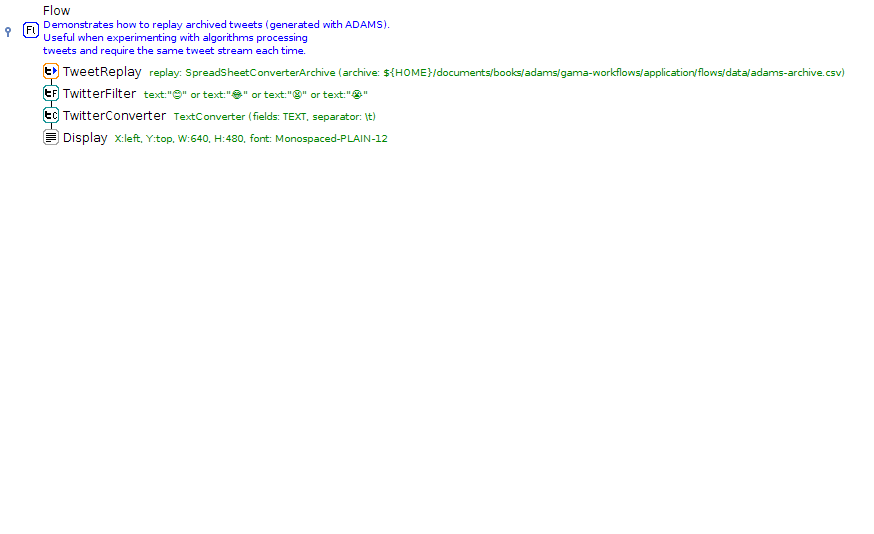
\includegraphics[width=10.0cm]{images/replay_and_filter_tweets-flow.png}
  \caption{Flow for replaying and filtering tweets from a CSV archive, using simple textual output.}
  \label{replay_and_filter_tweets-flow}
\end{figure}

\begin{figure}[htb]
  \centering
  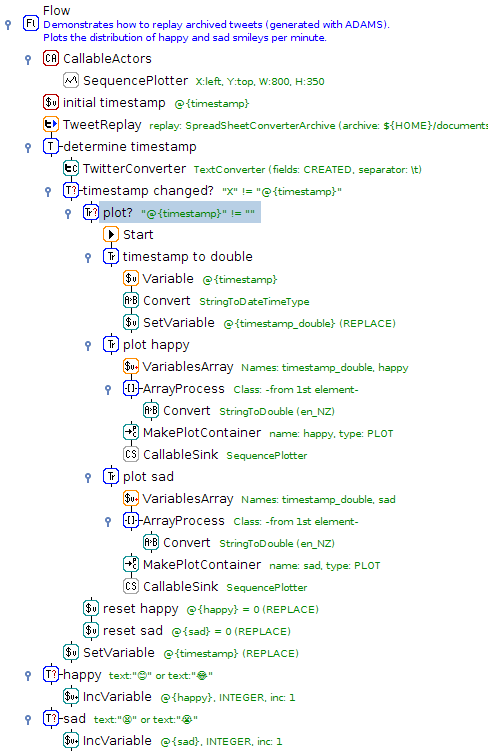
\includegraphics[width=8.0cm]{images/replay_and_filter_tweets2-flow.png}
  \caption{Flow for replaying and filtering tweets from a CSV archive, displaying mood distribution per minute.}
  \label{replay_and_filter_tweets2-flow}
\end{figure}

\begin{figure}[htb]
  \centering
  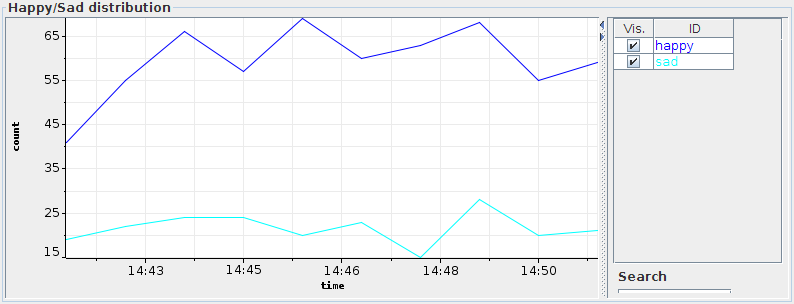
\includegraphics[width=10.0cm]{images/replay_and_filter_tweets2-output.png}
  \caption{Visualization of mood distribution per minute (``happy'' and ``sad'' smiley counts).}
  \label{replay_and_filter_tweets2-output}
\end{figure}

\begin{figure}[htb]
  \centering
  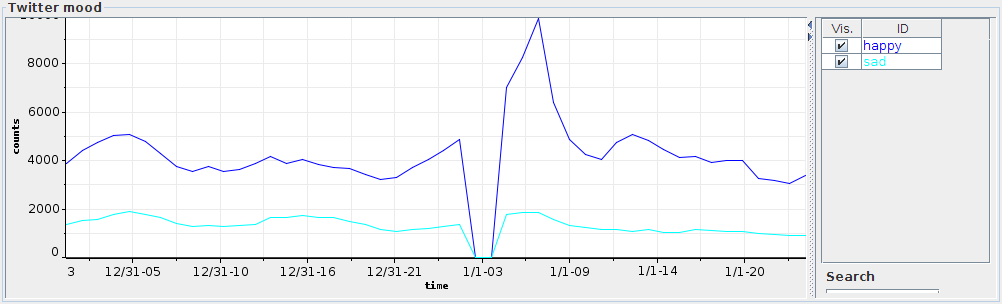
\includegraphics[width=10.0cm]{images/twitter_mood.png}
  \caption{Visualization of mood distribution per hour over New Years 2013/2014 (``happy'' and ``sad'' smiley counts).}
  \label{twitter_mood}
\end{figure}

\section{Visualizing tweets}
TODO

\subsection{Analysis}
TODO

\begin{figure}[htb]
  \centering
  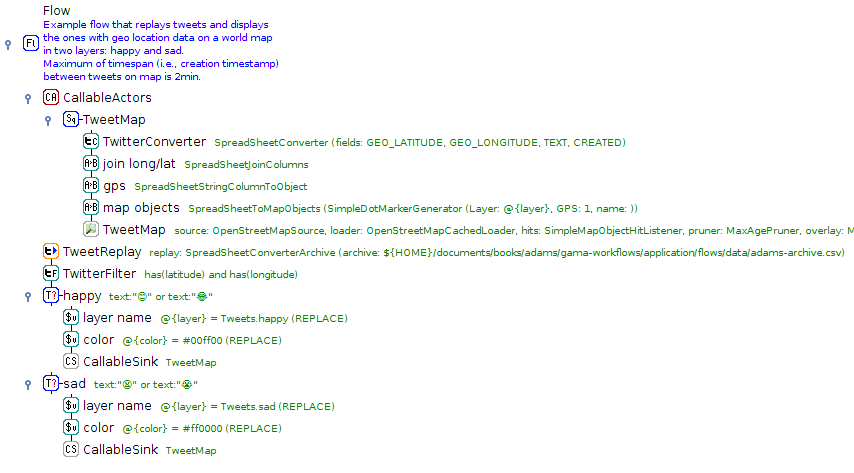
\includegraphics[width=12.0cm]{images/visualize_tweets-archive-flow.png}
  \caption{Flow for visualizing tweets archive.}
  \label{visualize_tweets-archive-flow}
\end{figure}

\begin{figure}[htb]
  \centering
  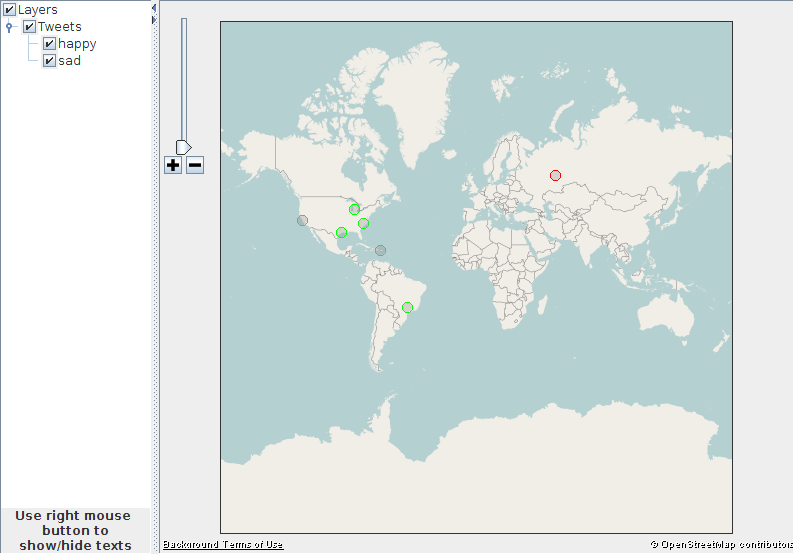
\includegraphics[width=10.0cm]{images/visualize_tweets-archive-output.png}
  \caption{Flow for visualizing tweets archive.}
  \label{visualize_tweets-archive-output}
\end{figure}

\subsection{Real-time visualization}
TODO

\begin{figure}[htb]
  \centering
  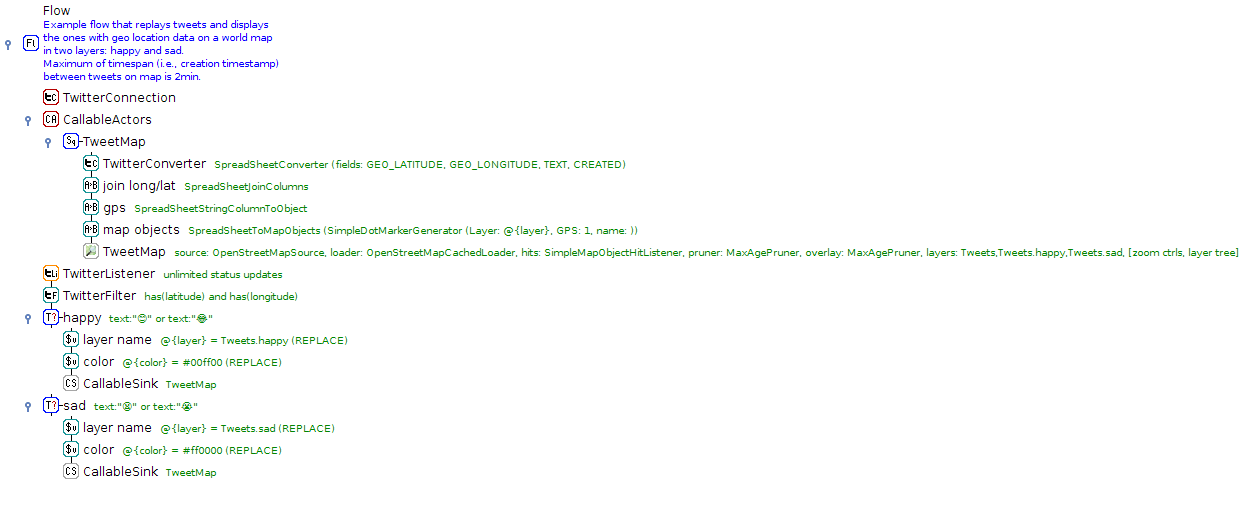
\includegraphics[width=12.0cm]{images/visualize_tweets-realtime-flow.png}
  \caption{Flow for visualizing tweets in real-time.}
  \label{visualize_tweets-realtime-flow}
\end{figure}

\end{document}
